% =====================================
% Purpose: Create a Robert Bringhurst style thesis paper using the 
% classicthesis package and some custom enhancements - this is 
% the default template for most of my documents
% =====================================

% =====================================
% Document Class and main packages
% =====================================

\documentclass[10pt,a4paper, hidelinks]{article} % KOMA-Script article scrartcl
\usepackage[nochapters, pdfspacing]{classicthesis} % [nochapters] [drafting] (puts date/time at bottom) [beramono] (changed mono spaced font)

% =====================================
% Packages in Use
% =====================================

%Math Packages
\usepackage{amsmath}
\usepackage{amsfonts}
\usepackage{amssymb}
\usepackage{nicefrac} % For typsetting inline fractions
\usepackage{mathtools} % For substack and mathclap (underbrace helper commands)
\usepackage{algpseudocode}
\usepackage{tcolorbox}
%\usepackage[]{algorithm2e}

%% Typography enhancements
\usepackage{microtype} % For awesome typographical improvements
\usepackage{booktabs} % Pretty \begin{tabular}
\usepackage{multicol} % For pretty multi-columns enviroments
\usepackage{xspace} % For use in a command to ensure proper spacing
%\usepackage{geometry} %uncomment this is you want full page documentation
\usepackage{graphicx} % for allowing pictures
\usepackage{float} % For the purpose of adding \begin{figure} [H]
\usepackage{lipsum} % For adding filler text
\usepackage{wasysym} % For the \newmoon command for the legal blobs

% For commenting on incomplete or new items
\usepackage{todonotes} % \missingfigure{} is the best command

% For inclusion of PDFs in the document \includepdf[pages={3,{},8-11,15}]{example.pdf}
% This will include page 3, a blank page, 8,9,10,11, and 15
% you can set this to draft to get boxes or final to get the default which includes
% the pages
% Options:
% 	fitpaper: Use this to insert the page as is - otherwise items are scaled to page
% 	rotateoversize: Attempt to rotate oversized pages and scale them
\usepackage[final]{pdfpages}

% =====================================
% Graphics 
% =====================================

% For quick graphics insert -- Full Line --
\newcommand{\qpic}[2]{
\begin{figure}[H]
\centering
\includegraphics[width=1\linewidth]{./#1}
\caption{#2}
\label{fig:#1}
\end{figure}
}

% For quick graphics insert -- Normal Size --
\newcommand{\qpics}[2]{
\begin{figure}[H]
\centering
\includegraphics[width=0.7\linewidth]{./#1}
\caption{#2}
\label{fig:#1}
\end{figure}
}

% =====================================
% Custom Macros that make life easier
% =====================================

% Description Enviroment Item Helper Commands
\newcommand{\im}[1]{\item[#1] \xspace}
\newcommand{\imp}[1]{\item[(#1)] \xspace}

% Auto-commas for long nominal and dollar amounts
\RequirePackage{siunitx}
\newcommand{\commasep}[1]{\num[group-separator={,}]{#1}}
\newcommand{\money}[1]{\$\commasep{#1}}
\usepackage{forest}
% Borrowing from tufte, this is the \newthought command that is 
% often used to bring about the change from one subsubsection
% to another and is a good way to bring things up logically into smaller
% bites
\newcommand{\newthought}[1]{
\vspace{11pt} \noindent
\spacedlowsmallcaps{#1}
}

% Code for the fast creation of bullet lists
\newcommand{\qb}[1]{\begin{itemize} #1 \end{itemize}}

% Code to produce spaced small caps in real text
\newcommand{\mysmallcaps}[1]{\spacedlowsmallcaps{#1}\xspace}

% Legal blobbing for reminding oneself to include information there: [<circle>]
\newcommand{\legalblob}{\ensuremath{\left[\newmoon\right]}}

% Simple math macros for probablility and expectations that are very common for math homework
\newcommand{\p}{\ensuremath{\mathbb{P}}\xspace}
\newcommand{\expt}[1]{\ensuremath{\mathbb{E}}\left[#1\right]\xspace}
\newcommand{\myvec}[1]{\underset{\sim}{#1}}
\newcommand{\myexp}[1]{\exp\left( #1\right) }

% =====================================
% For handling code blocks and other text
% =====================================

% Code to handle inputting code segments in R
% To import code use: \lstinputlisting[language=R]{h1code.r}
% To add code in-line use \begin{lstlisting}[language = {}] 
% \lstinputlisting[language={}]{file.txt} for  unformatted code
\usepackage{listings} 
\lstset{language=R} 
\usepackage{color}
\definecolor{mygreen}{rgb}{0,0.6,0}
\definecolor{mygray}{rgb}{0.5,0.5,0.5}
\definecolor{mymauve}{rgb}{0.58,0,0.82}
\definecolor{harvard}{RGB}{145,60,58}

\lstset{ %
  backgroundcolor=\color{white},   % choose the background color; you must add \usepackage{color} or \usepackage{xcolor}
  basicstyle=\footnotesize,        % the size of the fonts that are used for the code
  breakatwhitespace=false,         % sets if automatic breaks should only happen at whitespace
  breaklines=true,                 % sets automatic line breaking
  captionpos=b,                    % sets the caption-position to bottom
  commentstyle=\color{mygreen},    % comment style
  deletekeywords={...},            % if you want to delete keywords from the given language
  escapeinside={\%*}{*)},          % if you want to add LaTeX within your code
  extendedchars=true,              % lets you use non-ASCII characters; for 8-bits encodings only, does not work with UTF-8
  frame=single,	                   % adds a frame around the code
  keepspaces=true,                 % keeps spaces in text, useful for keeping indentation of code (possibly needs columns=flexible)
  keywordstyle=\color{blue},       % keyword style
  language=R,                 % the language of the code
  otherkeywords={*,...},            % if you want to add more keywords to the set
  numbers=left,                    % where to put the line-numbers; possible values are (none, left, right)
  numbersep=5pt,                   % how far the line-numbers are from the code
  numberstyle=\tiny\color{mygray}, % the style that is used for the line-numbers
  rulecolor=\color{black},         % if not set, the frame-color may be changed on line-breaks within not-black text (e.g. comments (green here))
  showspaces=false,                % show spaces everywhere adding particular underscores; it overrides 'showstringspaces'
  showstringspaces=false,          % underline spaces within strings only
  showtabs=false,                  % show tabs within strings adding particular underscores
  stepnumber=2,                    % the step between two line-numbers. If it's 1, each line will be numbered
  stringstyle=\color{mymauve},     % string literal style
  tabsize=2,	                   % sets default tabsize to 2 spaces
  title=\lstname                   % show the filename of files included with \lstinputlisting; also try caption instead of title
}

% =====================================
% Beginning the main document
% =====================================

\begin{document}
\pagestyle{plain} 
\title{\color{harvard}\rmfamily\normalfont {\Huge  \spacedallcaps{Learning the Madness}} \\ \vspace{-.4cm}\hfill\\ {\LARGE \textit{NCAA March Madness Predictions}}}
\author{\textsc{Andrei Kopelevich}\\ \textsc{Mark Kurzeja}\\ \textsc{Eli Schultz} }
\date{} % no date or \today if you want to insert a date

\maketitle

\mbox{}
\vfill

\begin{center}
	\large \color{harvard}   \textit{Professor Long Nguyen - Stats 503} \\ \spacedlowsmallcaps{April 16$^{th}$, 2018} 
\end{center}
\thispagestyle{empty}
\newpage

\hfill
\vspace{1cm}\hfill

\begin{abstract}
	Every year, millions of people fill out March Madness brackets in attempt to predict the outcome of the NCAA men's basketball tournament. A big part of the draw is that the tournament is notoriously difficult to predict, and predicting a perfect bracket is so improbable that Warren Buffet, a US investor, annually offers \$1MM a year for life to any of his employees who can predict the exact outcome of the tournament. Many algorithms for predicting the tournament attempt to predict results at the individual game level, based on how teams match up with one another. We will instead focus on predicting how many rounds a team will progress in the tournament based on its performance over the course of the preceding season, with the goal of building stable and consistent predictions of tournament outcomes.
\end{abstract}
\tableofcontents
\thispagestyle{empty}
\newpage

 \pagenumbering{arabic} 
\section{Background}
\subsection{Problem Description}
After all regularly scheduled NCAA basketball games are concluded in mid-March, 68 teams are selected to participate in the NCAA tournament. Every game is single elimination, meaning that as soon as a team loses it is eliminated from the tournament. Eight of the 68 teams originally chosen have to compete in so-called play-in games, after which 64 teams remain. We will follow the same framework as that followed by most bracket prediction contests and concern ourselves here with predicting how teams will perform once the field has been narrowed down to 64 contenders. At this point there are $2^{32} \cdot 2^{16} \cdot 2^8 \cdot 2^4 \cdot 2^2 \cdot 2 = 2^{63}$ possible outcomes, which gives one an idea of the scope of this challenge. Predicting a perfect bracket may be impossible, but we will see how close we can get.

\subsection{The Data Set}

The first step in our analysis was gathering data. There are many decades of team performance data available on the Sports Reference college basketball website free of charge \cite{bballsite}. However, in recent years a number of more advanced metrics have been devised that have been shown to more accurately capture a team's strength. Since this data is only available starting from 1993, we limited our analysis to that timeframe. Our working data set ultimately consisted of 12 continuous quantitative predictors, and one categorical response corresponding to the number of victories a team had in the tournament (ranging from 0 for a team that lost immediately to 6 for a national champion).

\subsubsection{Feature Description}

The predictors can be thought of as belonging to six broad buckets corresponding to aspects of a team performance:

\begin{itemize}
	\item Winning percentage, strength of schedule (SOS) and simple rating system (SRS) are all holistic measures.
	\item Free throw attempt rate (ft\_rate0), free throw attempts per field goal attempt (fta\_per\_fga\_pct),  three-point attempts per field goal attempt (fg3a\_per\_fga\_pct), and assist rate (ast\_pct) all help classify a team's offensive playing style. The idea is that three-point shots are high risk and high reward while free throws are low risk and low reward. Thus teams that attempt more three point shots may have more variable performances from game to game, while teams that attempt more free throws may be more consistent. Teams with higher assist rates should be expected to play more collaboratively, while teams with low assist rates rely more on strong individual performances.
	\item Total rebound percentage (trb\_pct) captures how well a team recovers the ball following shots missed by either themselves or their opponents.
	\item True shooting percentage (ts\_pct) and effective field goal percentage (efg\_pct) both capture how well a team shoots the ball.
	\item Turnover percentage (tov\_pct) captures how well a team is able to avoid allowing the other team to take the ball away (better teams should generally have lower turnover percentages).
	\item Block percentage (blk\_pct)  captures how well a team is able to block the other team's shots.
\end{itemize}

It is worth noting that the vast majority of these statistics capture how well a team performs offensively.  

\section{Preliminary Data Exploration}

\subsection{Data Exploration and Visualization}

\subsubsection{Data Summaries and Discussion}

We began by performing data exploration and visualization, as well as dimension reduction, to inform our analysis.

Summaries of the predictors are provided below.



\begin{table}[!htbp] \centering 
	\caption{} 
	\label{} 
	\begin{tabular}{@{\extracolsep{5pt}}lccccc} 
		\\[-1.8ex]\hline 
		\hline \\[-1.8ex] 
		Statistic & \multicolumn{1}{c}{N} & \multicolumn{1}{c}{Mean} & \multicolumn{1}{c}{St. Dev.} & \multicolumn{1}{c}{Min} & \multicolumn{1}{c}{Max} \\ 
		\hline \\[-1.8ex] 
		winlosspct & 1,636 & 0.717 & 0.095 & 0.367 & 0.974 \\ 
		srs & 1,636 & 11.298 & 8.160 & $-$17.130 & 34.800 \\ 
		sos & 1,636 & 3.989 & 5.677 & $-$14.180 & 13.010 \\ 
		fta\_per\_fga\_pct & 1,636 & 0.388 & 0.050 & 0.225 & 0.654 \\ 
		fg3a\_per\_fga\_pct & 1,636 & 0.317 & 0.058 & 0.141 & 0.532 \\ 
		ts\_pct & 1,636 & 0.550 & 0.025 & 0.451 & 0.620 \\ 
		trb\_pct & 1,636 & 51.808 & 2.384 & 42.400 & 61.100 \\ 
		ast\_pct & 1,636 & 56.332 & 5.291 & 40.300 & 74.000 \\ 
		blk\_pct & 1,636 & 8.961 & 2.986 & $-$2.200 & 20.400 \\ 
		efg\_pct & 1,636 & 0.516 & 0.026 & 0.412 & 0.598 \\ 
		tov\_pct & 1,636 & 16.697 & 1.954 & 2.300 & 23.200 \\ 
		ft\_rate0 & 1,636 & 0.271 & 0.037 & 0.160 & 0.430 \\ 
		\hline \\[-1.8ex] 
	\end{tabular} 
\end{table} 

At a high level, the first three predictors provide a good sanity check in that they suggest that  teams in the tournament are generally better than average teams. The first quartile for winning percentage (percentage of games that a given team won) is well above 50\% for the teams in our data set. Our teams also generally have strength of schedule and simple rating system scores well above zero, which is to be expected given that those metrics are designed such that an average team will have a score around zero. It may seem a bit strange at first that stronger teams will tend to have a better SOS score, but this can be explained by the fact that strong teams tend to be in the same conferences as other strong teams, and therefore play other strong teams more frequently.

It is also worth noting that a number of the predictors have unusually large and/or small outliers. To visualize high-level trends in the predictors, boxplots of each of the predictors for each of the six tournament win groups are provided below. Some of the predictors, such as assist percentage and the two free-throw related predictors, seem to be fairly similarly distributed across the six groups. However, there are a number of pronounced patterns. For instance, more successful tournament teams generally tend to much higher win-loss percentages, SRS, and SOS scores. This is also true, although to a lesser extent, for true shooting percentage, effective field goal percentage, total rebound percentage, and block percentage. Similarly, more successful teams tend to have lower turnover rates. 

\begin{figure}[H]
	\centering
	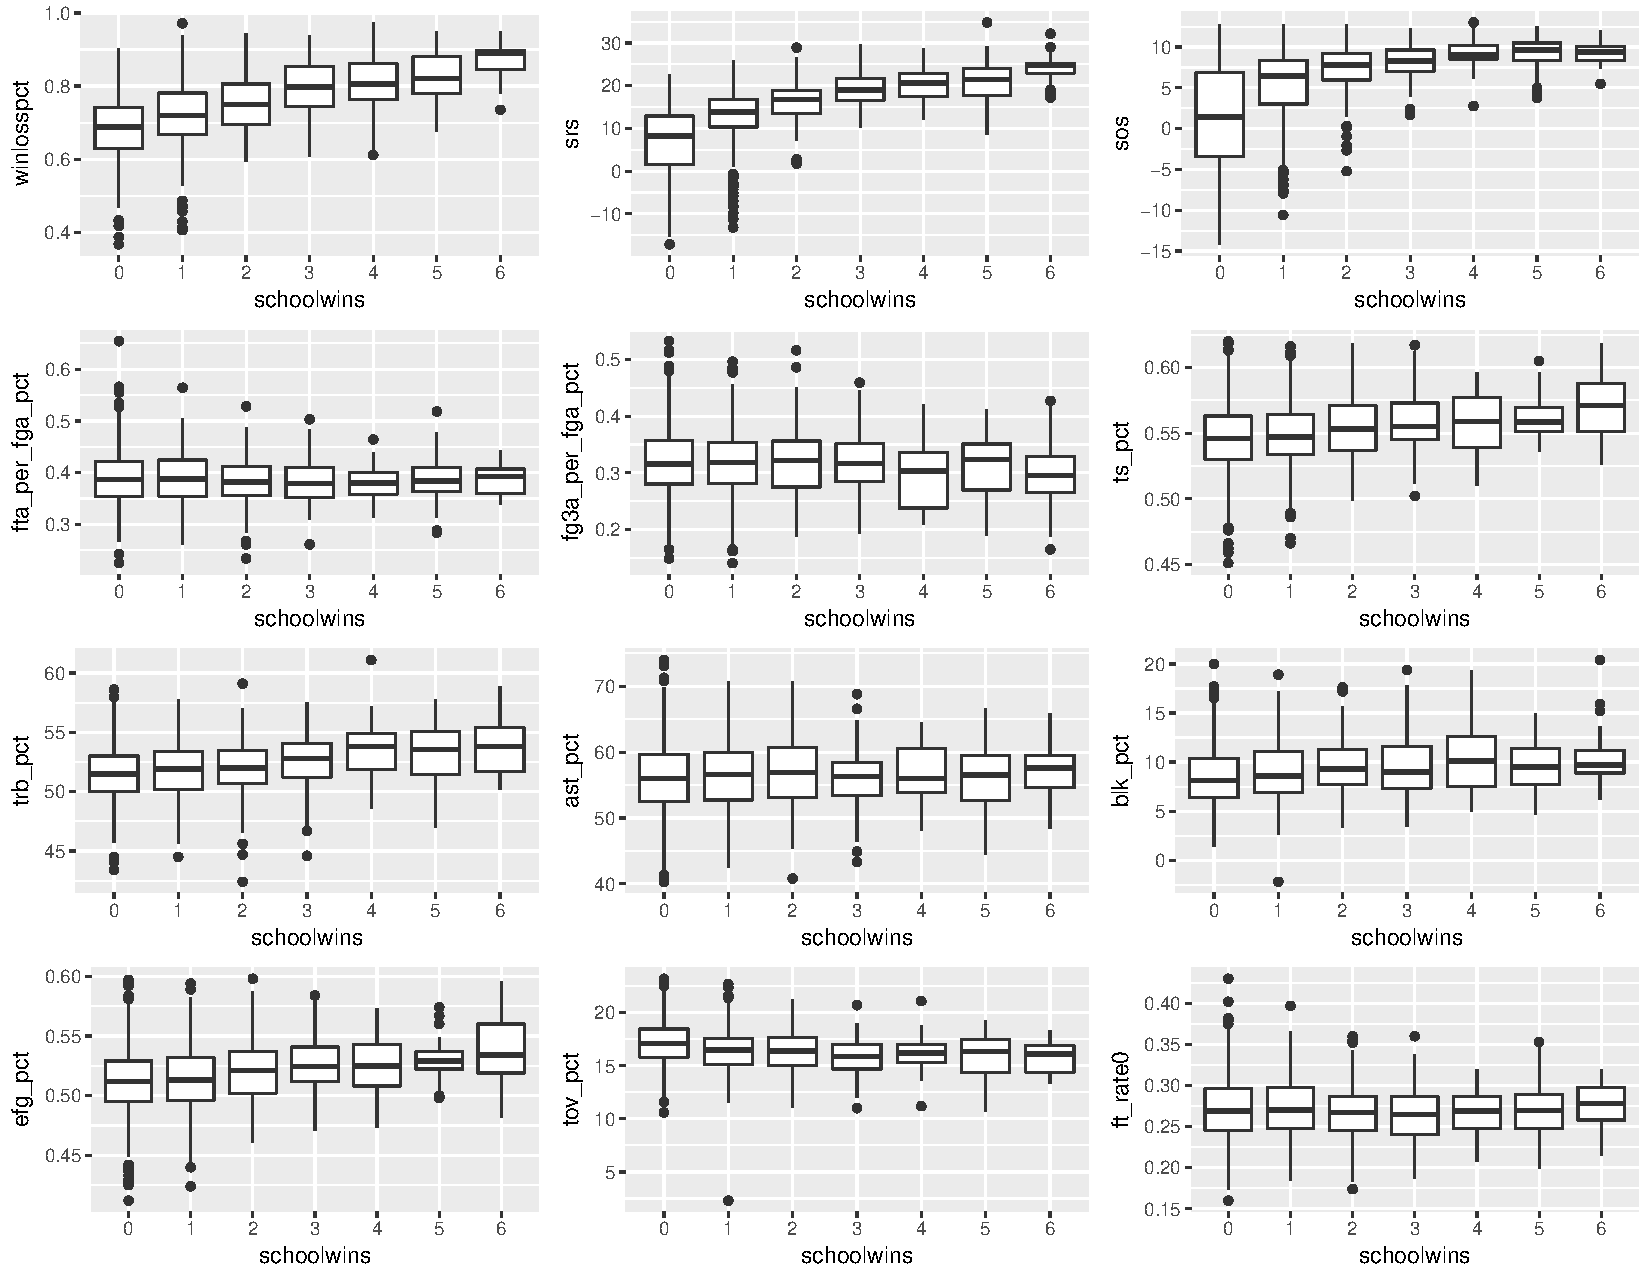
\includegraphics[width=1\linewidth]{../fig/RayleighsWetDream.pdf}
	\caption{caption goes here}
	\label{fig:rayleighwetdream}
\end{figure}

\subsubsection{Discussion of Correlations}

A pairwise scatterplot of the predictors is provided below. Many of the correlations are relatively small. Unsurprisingly, in some cases where two predictors belong to the same bucket (per the framework above) we notice very strong correlations. Effective field goal percentage and true shooting percentage are the most strongly correlated predictors ($r \approx 0.96$), which is to be expected given that both measure how well a team shoots the ball. Free throw rate and free throw attempts per field goal attempt ($r \approx 0.922$) both capture how often a team tends to shoot free throws in slightly different ways. Finally, the strong correlations between SRS and wining percentage ($r \approx 0.518$) and SRS and SOS ($r \approx 0.867$) reflect the fact that SRS is meant to capture team performance, adjusted for strength of schedule.

\begin{figure}[H]
	\centering
	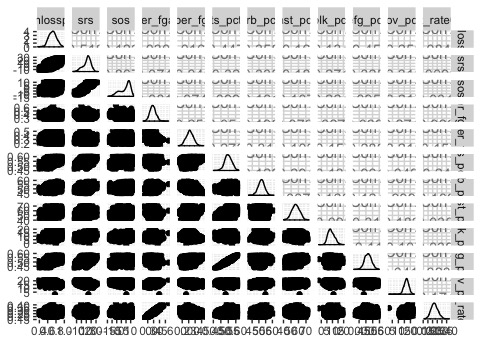
\includegraphics[width=1\linewidth]{../fig/MoneyMaker.pdf}
	\caption{caption goes here}
	\label{fig:ggpairs}
\end{figure} 

However, there are a few other correlations that are much weaker, but perhaps a little more interesting for the purposes of our model. For instance, there is a weak negative correlation between rebounding percentage and free throw attempts per field goal attempt ($r \approx -0.311$), a correlation which does not seem to have an obvious intuitive explanation based on the buckets outlined above. Similarly, both true shooting percentage ($r \approx 0.273$) and effective field goal percentage ($r \approx 0.282$) were weakly correlated with three point attempts per field goal attempt.

\subsubsection{Dimension Reduction}

Overall, the presence of these correlations suggests that it may be useful to perform PCA in an attempt to reduce overall dimensionality for the purposes of preliminary investigation and visualization.

A skree plot of percentage of variance explained against number of principal components used is shown below. 

\begin{figure}[H]
	\centering
	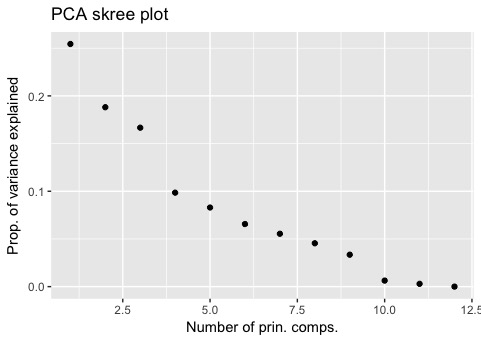
\includegraphics[width=0.7\linewidth]{../fig/Skreeeeee}
	\caption{caption goes here}
	\label{fig:Skreeeeee}
\end{figure}

From a numeric standpoint, there is no obvious cutoff here. We do see that that the fourth principal component explains much less of the variance than the third, but it still explains about 10\% of the variance, and thus cannot be easily discarded. However, for visualization purposes we will look at plots of the data projected onto all three possible pairwise combinations of the first three principal components.

\begin{figure}[H]
	\centering
	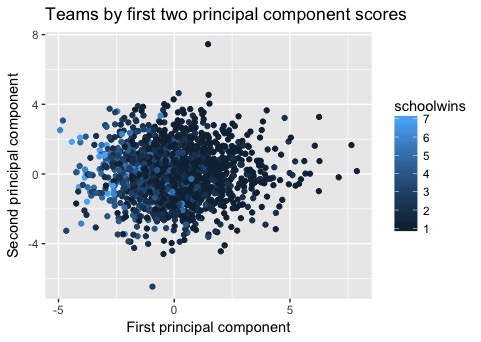
\includegraphics[width=0.7\linewidth]{../fig/PrinComps}
	\caption{caption goes here}
	\label{fig:princomps}
\end{figure}


While we do not necessarily observe perfect clustering corresponding to each of the possible win totals, it is encouraging to see that in general the principal components seem to separate better-performing teams (represented by the lighter colors above) from weaker teams (represented by the darker blue above). 

Although it only explains roughly 25\% of the variance in the data, the first principal component in particular seems to do a fairly good job of differentiating weak teams from strong ones, with teams that advanced further in the tournament tending to have lower scores for that component. The first principal component can roughly be interpreted as a negative average of winning percentage, SOS, SRS, effective field goal percentage, and true shooting percentage (although there are small contributions from a few other variables as well). In context, this result suggests that just looking at team's overall performance and ability to shoot gives a decent first order idea of whether or not it will perform well in the tournament.

\subsection{Clustering}
\subsubsection{Overview}
As noted above, the first two principal components showed some evidence of underlying clustering in the data corresponding to tournament wins. We will explore this idea further here by applying selected clustering algorithms to see whether such a clustering structure can be detected. We begin by fitting a mixture model to our data.

Plotting BIC as a function of the number of clusters $k$ for a mixture model gives us an estimate for the optimal number of clusters to use.

\begin{figure}[H]
	\centering
	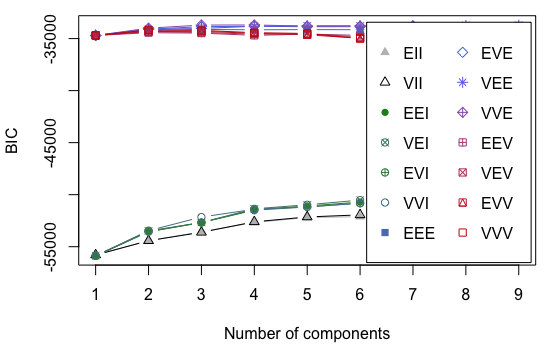
\includegraphics[width=0.7\linewidth]{../fig/sonofaBIC}
				\caption{BIC vs. k}
\end{figure}

This turns out to be four, for a VVE model.

\subsubsection{K-means}

\begin{figure}[H]
	\centering
	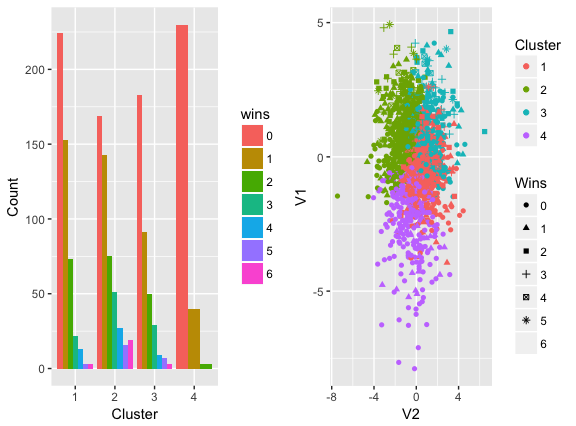
\includegraphics[width=0.7\linewidth]{../fig/clusterfun}
			\caption{Wins by cluster and 2D MDS plot of clusters, k-Means}
\end{figure}

K-means clustering over four categories produces encouraging results similar to those of the PCA performed above. While three of the clusters seem to have generally similar proportions of teams from each win category represented, once cluster consists mainly of teams that perform very poorly.  These results are consistent across different random initialization conditions for the K-means algorithm. While three groups show similar win rates, one is a laggard.

\begin{figure}[H]
	\centering
	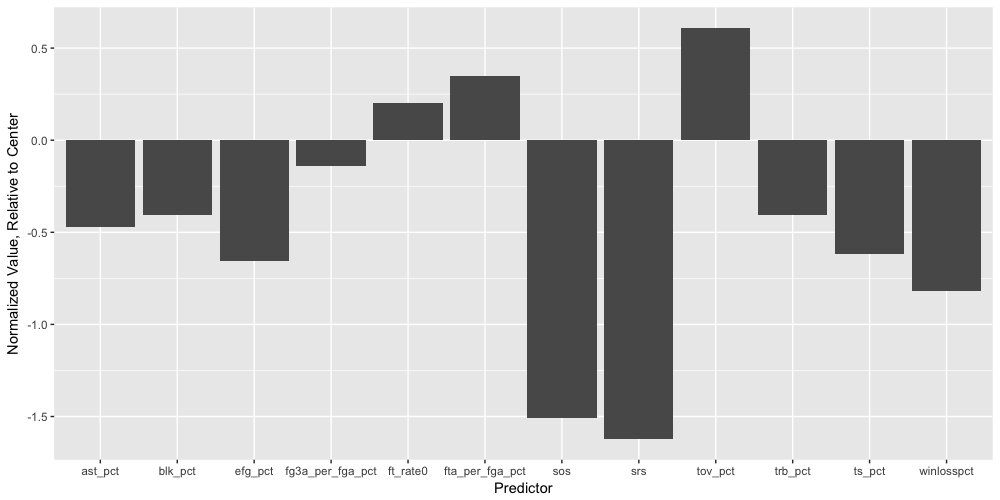
\includegraphics[width=0.7\linewidth]{../fig/weakclusterk}
		\caption{Standardized mean difference from full data, k-Means}
\end{figure}

Relative to the general data, the observations in this cluster have substantially lower values of SRS and SOS, with less extreme negative differences from the norm in assist rate, block rate, effective field goal percentage, rebounding rate, true shooting percentage, and win rates, along with a slightly higher than usual turnover percentage. All of these deviations are consistent with what would be expected for weaker teams. Therefore teams belonging to this cluster can be expected to perform poorly in the tournament.  The silhouette plot below gives us another way to explore the results of k-means.

\begin{figure}[H]
	\centering
	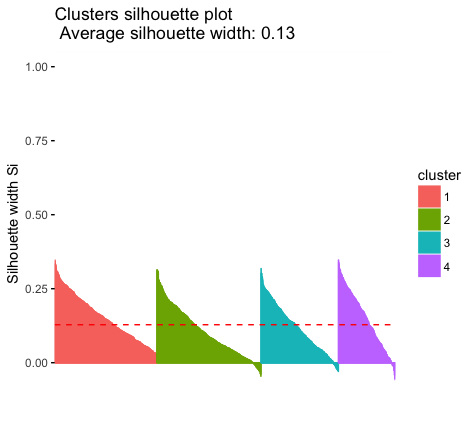
\includegraphics[width=0.5\linewidth]{../fig/kmeansil}
		\caption{Silhouette plot, k-Means}
\end{figure}

The clustering here appears somewhat ambiguous, with an average silhouette width of 0.13.  It is also a bit concerning that some of the weakest clusterings occur in the fourth category, which is the cluster identified above as potentially corresponding to weaker teams.

\subsubsection{Hierarchical Clustering}

\begin{figure}[H]
	\centering
	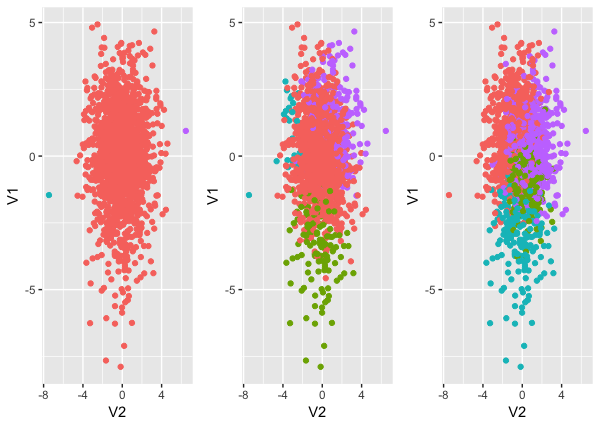
\includegraphics[width=0.7\linewidth]{../fig/areyouheigh}
		\caption{2D MDS plots of clusters: single linkage, complete linkage, and Ward's method, Euclidean distance}
\end{figure}

We next explore what hierarchical clustering can tell us about the data. When hierarchical clustering is performed using Euclidean distances and either complete linkage or Ward's method, we see a result fairly similar to that obtained from k-means.  Single linkage, however, maps everything except for two isolated observations into a single cluster. It appears that the heavy degree of noise in our dataset prevents a more meaningful clustering under the latter dissimilarity measure.

\begin{figure}[H]
	\centering
	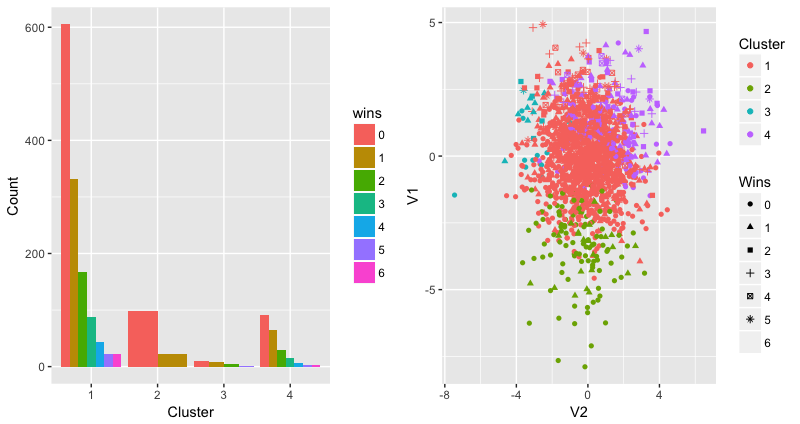
\includegraphics[width=0.7\linewidth]{../fig/comp1}
		\caption{Wins by cluster and 2D MDS plot of clusters, complete linkage, Euclidean distance}
\end{figure}

\begin{figure}[H]
	\centering
	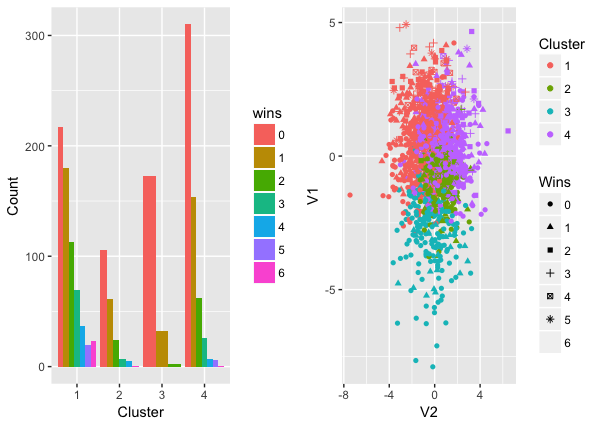
\includegraphics[width=0.7\linewidth]{../fig/ward1}
		\caption{Wins by cluster and 2D MDS plot of clusters, Ward's method, Euclidean distance}
\end{figure}

\begin{figure}[H]
	\centering
	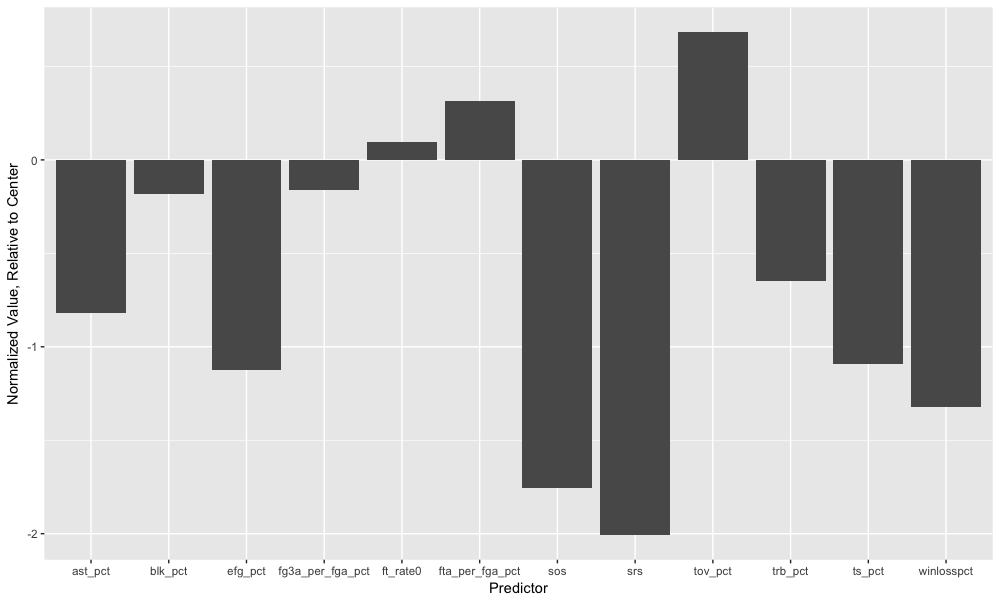
\includegraphics[width=0.7\linewidth]{../fig/compweak}
		\caption{Standardized mean difference from full data, complete linkage, Euclidean distance}
\end{figure}

\begin{figure}[H]
	\centering
	\includegraphics[width=0.7\linewidth]{"../fig/wardweak"}
		\caption{Standardized mean difference from full data, Ward's method, Euclidean distance}
\end{figure}


As noted above, the complete linkage and Ward's method clusters are very similar to the k-means clusters we obtained, although in the case of Ward's method one cluster contains a majority of the data. Once again, one of the clusters contains mostly teams that would be expected to perform poorly from a conceptual standpoint. This pattern is particularly extreme when using complete linkage.

\begin{figure}[H]
	\centering
	\includegraphics[width=0.5\linewidth]{"../fig/compsil"}
		\caption{Silhouette plot, complete linkage, Euclidean distance}
\end{figure}

\begin{figure}[H]
	\centering
	\includegraphics[width=0.5\linewidth]{"../fig/wardsil"}
		\caption{Silhouette plot, Ward's method, Euclidean distance}
\end{figure}

The silhouettes for these methods show much more ambiguity than in k-means: complete linkages have an average width of 0.07, and Ward's method gives an average width of .08, both with striking potential for misclustering in clusters 1 and 4.  On the whole, these appear to be less suitable than the clusters obtained from K-means.

Extending this analysis via alternative distance measures produces highly consistent results.  Changing the distance metric to Manhattan or Gower distances produced no meaningful changes in the the clusters and saw lower average silhouette widths.  These results have been omitted for the sake of brevity and available on request.

\subsubsection{Mixture Modeling}

Returning to our original mixture model, recall that BIC was maximized for a VVE model with four components.  The components will have proportions 28.5\%, 5.91\%, 33.67\%, and 31.86\%, and means described by the table of vectors below.

\begin{table}[ht]
	\centering
	\begin{tabular}{rrrrr}
		\hline
		& 1 & 2 & 3 & 4 \\ 
		\hline
		winlosspct & 0.38 & -0.61 & -0.07 & -0.16 \\ 
		srs & 0.68 & -0.99 & -0.91 & 0.53 \\ 
		sos & 0.56 & -0.90 & -1.02 & 0.74 \\ 
		fta\_per\_fga\_pct & -0.09 & 0.56 & -0.01 & -0.01 \\ 
		fg3a\_per\_fga\_pct & -0.04 & 0.41 & 0.09 & -0.13 \\ 
		ts\_pct & 0.05 & 0.05 & -0.00 & -0.05 \\ 
		trb\_pct & 0.24 & -0.59 & -0.15 & 0.05 \\ 
		ast\_pct & -0.04 & 0.02 & -0.10 & 0.14 \\ 
		blk\_pct & 0.48 & -0.18 & -0.34 & -0.04 \\ 
		efg\_pct & 0.08 & -0.00 & 0.01 & -0.08 \\ 
		tov\_pct & -0.22 & 0.36 & 0.21 & -0.09 \\ 
		ft\_rate0 & -0.08 & 0.46 & -0.03 & 0.01 \\ 
		\hline
	\end{tabular}
\end{table}

The third component appears roughly consistent with the characteristics of weak clusters we observed under previous methods.  This notion is confirmed by plotting the clusters against wins and 2D MDS plots per earlier.  

\begin{figure}[H]
	\centering
	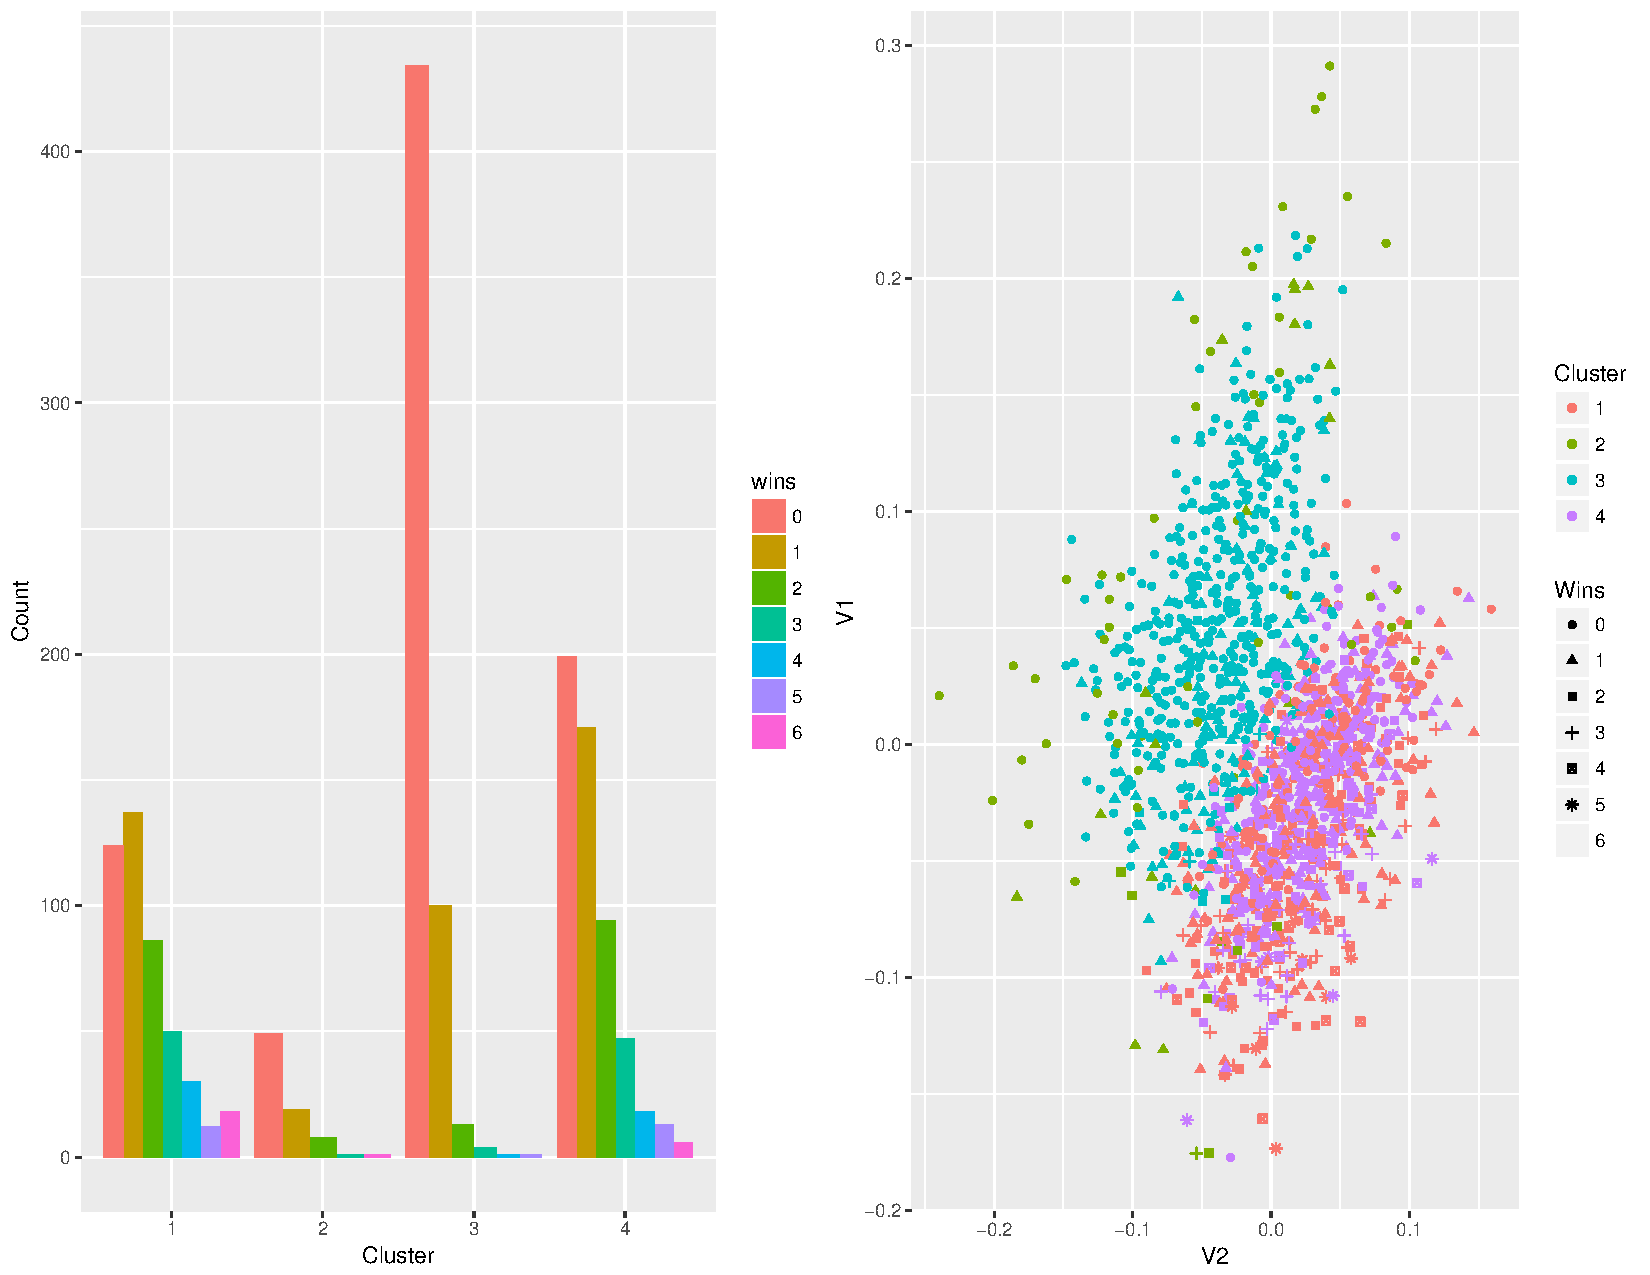
\includegraphics[width=0.7\linewidth]{../fig/sirmixalot}
	\caption{Wins by cluster and 2D MDS plot of clusters, Mixture Model}
\end{figure}

\begin{figure}[H]
	\centering
	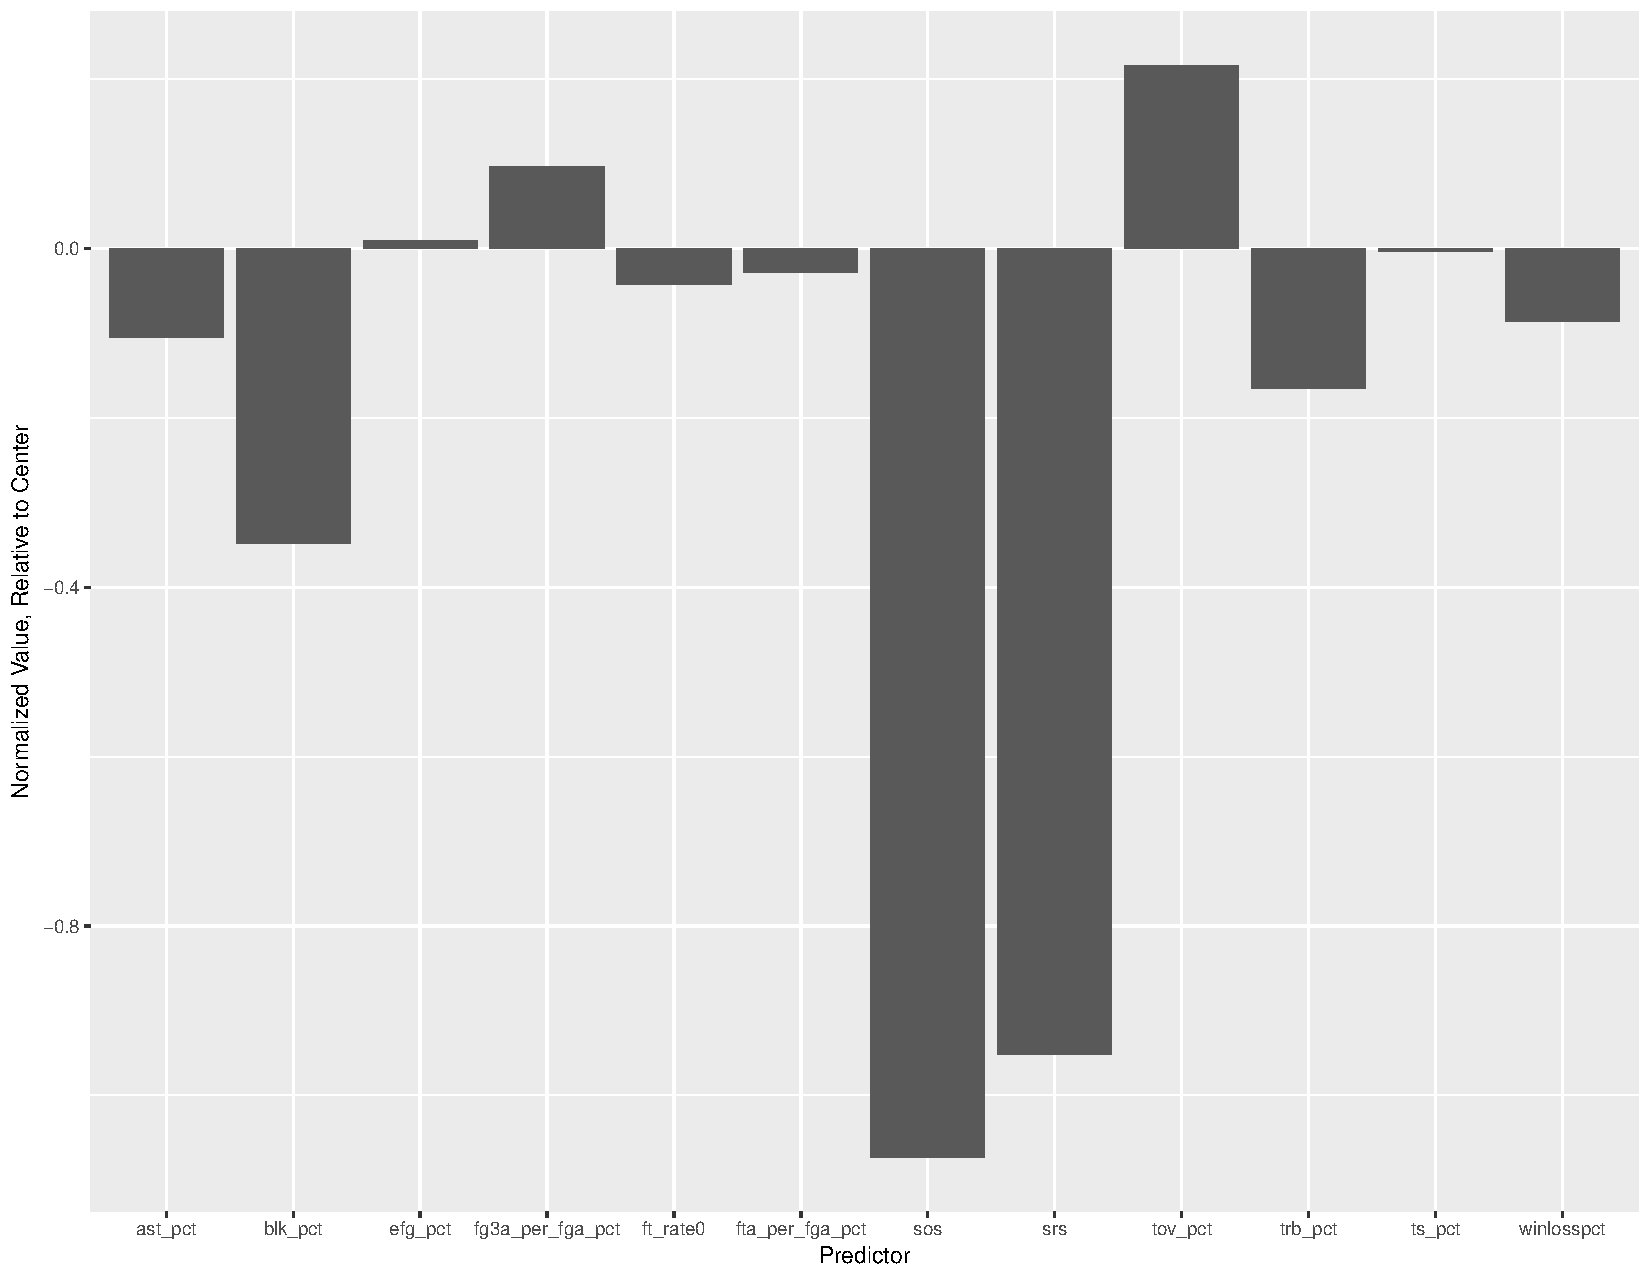
\includegraphics[width=0.7\linewidth]{../fig/mixweak}
	\caption{Standardized mean difference from full data, Mixture Model}
\end{figure}

As we can see, the third components relationship with winning games, the MDS components, and the predictors all appear highly similar to the least-winning cluster or clusters observed in the previous methods.

\begin{figure}[H]
	\centering
	\includegraphics[width=0.5\linewidth]{"../fig/mixsil"}
	\caption{Silhouette plot, Mixture Model}
\end{figure}

The silhouette plot of our mixture model shows the lowest average silhouette width, tied with the Ward's method and Gower distance pair in a hierarchical clustering.

In summary, across three different methods and variations within, we see a relatively consistent clustering showing teams with very low SRS and SOS, below-average Blocks, Rebounds, and Win rates, and above typical Turnover Percentage are associated with failing to pass the Sweet 16.  Of our methods, k-Means appeared to return the least ambiguous clusters.

\subsection{Ordinal Regression}
\subsubsection{Overview}
When looking at our problem, we ran into an issue with the domain of the response variable (how many games a team will win in the tournament). In particular, our response variable is neither continuous (since it takes on only integer values and is bounded), nor is this a pure classification problem (because their is a natural ordering in the response). As a result, we needed to run an ordinal regression, at least at the outset, to see how well the data can be summarized with this approach before we moved on to more complicated models.  

%\subsubsection{Fitting the First Model}
%For the ordinal regression problem, we chose to use the \texttt{rstanarm polr} functions, as this allows us to view the posterior distributions of the coefficients, and determine the uncertainty that we have around each of our estimates. We chose to do the Bayesian variant of ordinal regression as sports data is notoriously noisy and most predictors will have little relationship with our outcome of interest. We needed to quantify errors more precisely as a result, and this method allowed us to do so. We began by standardizing the variables to avoid having the coefficients on different unit scales. We then excluded the teams names themselves to see if the other predictor variables can be used to discern performance. 
%
%After running the model, we ran the checks on the posterior distribution, and saw that each of the four chains used have converged, there were no divergences in any of the four chains, and the tree-depth was not hit on any of the iterations, signaling that the prior distribution on $R^2$ was sufficiently informative to ensure that the chains did not explore too far from the true posterior distribution\footnote{For information on how the prior distribution of $R^2$ or on the operation of \texttt{rstanarm}, please refer to the guide here: {\color{blue} \url{https://cran.r-project.org/web/packages/rstanarm/rstanarm.pdf}}}.
%
%The posterior distributions for the log-odds of the parameters are as follows:
%
%\begin{figure}[H]
%	\centering
%	\input{"../fig/polr_orig_coef.txt"}
%%	\caption{}
%\end{figure}
%
%Note that the coefficients are standardized. While the coefficients do not have interpretations that are as meaningful in the units of the problem, we can use their absolute magnitude, and whether their credible intervals contain zero, to discern variables relevance in improving the odds of moving from one round to the next. If a given credible interval contains zero, we can say that it is reasonably likely that $\exp(\beta_i) = 1$ which indicates that there is reason to believe that the odds ratio is equal to one. This is equivalent to saying that there is no significant change in the odds with the use of this coefficient.
%
%We also see that there are some pretty strong correlations between the effective field goal percentage, total shooting percentage, and other variables. We aim to reduce the multi-collinearity in the model by removing those terms that have significant correlation with one another, and then we refit the model. 

\subsubsection{Running the Model and Model Checking}
%\begin{figure}[H]
%	\centering
%	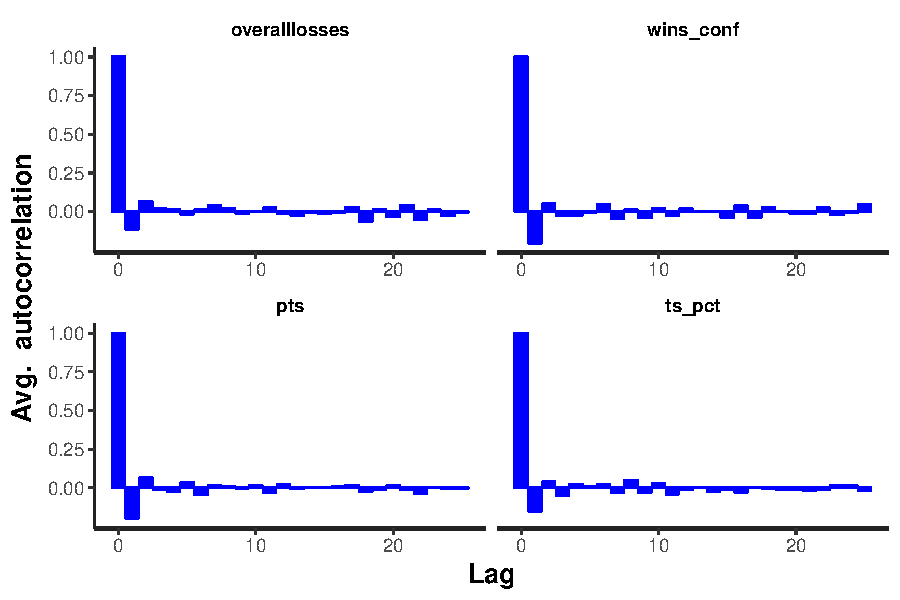
\includegraphics[width=.6\linewidth]{../fig/polr_autocorr}
%	\caption{The autocorrelation on all of the parameters looked similar to the auto-correlation above. We can see that the posterior was explored throughly and the chains did not get stuck for long in any one particular area. }
%	\label{fig:polr_autocorrelation}
%\end{figure}

The autocorrelation plots, posterior summary statistics, R-hat metric, and Hamiltonian Energy was checked to ensure that the posterior did indeed converge. There were no divergent chains and no chain hit the treedepth for the Stan algorithm. As a result, we are able to proceed with the analysis.


\begin{figure}[H]
	\centering
	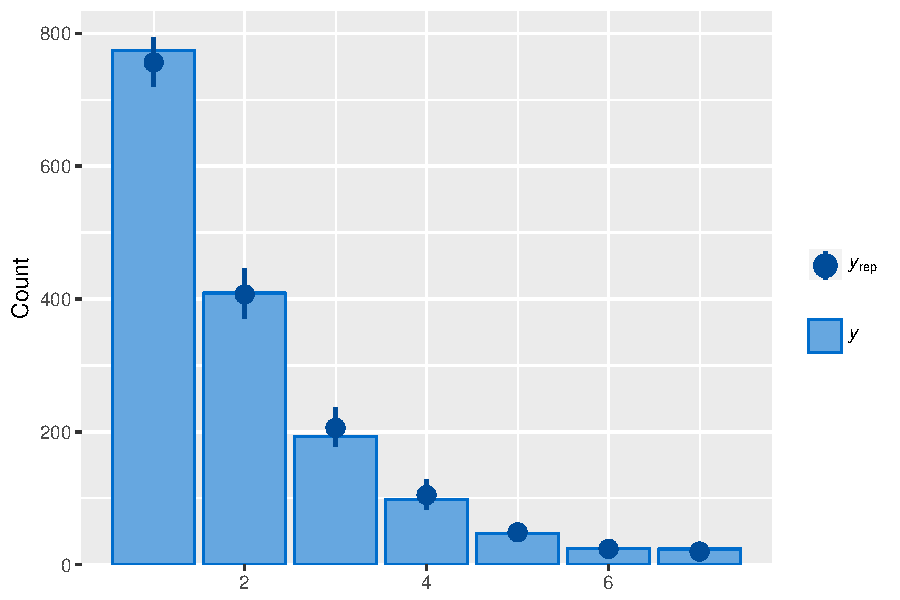
\includegraphics[width=0.7\linewidth]{../fig/polr_nonames_pp}
	\caption{This is a summary of the posterior predictive distribution for the first model that we ran with ordinal regression. We can see that the posterior is one of seven counts, and that if we run simulation from the predictive posterior, the resulting counds are in line with what we observed. This indicates that the model is capturing the frequency of the counts in its inference, which is important if we are not going to under bias or over bias any particular outcome. We can see especially at $wins = 0$ that the count is bias downwards, however, which makes sense given the imbalance of the representation of the zero count variables.}
	\label{fig:polrnonamespp}
\end{figure}


\subsubsection{The Model}

After removing the correlated variables, as we did above, we refit the model and obtained the following coefficients.

\begin{figure}[H]
	\centering
	\input{"../fig/polr_updated_coef.txt"}
	%	\caption{}
\end{figure}

\begin{figure}[H]
	\centering
	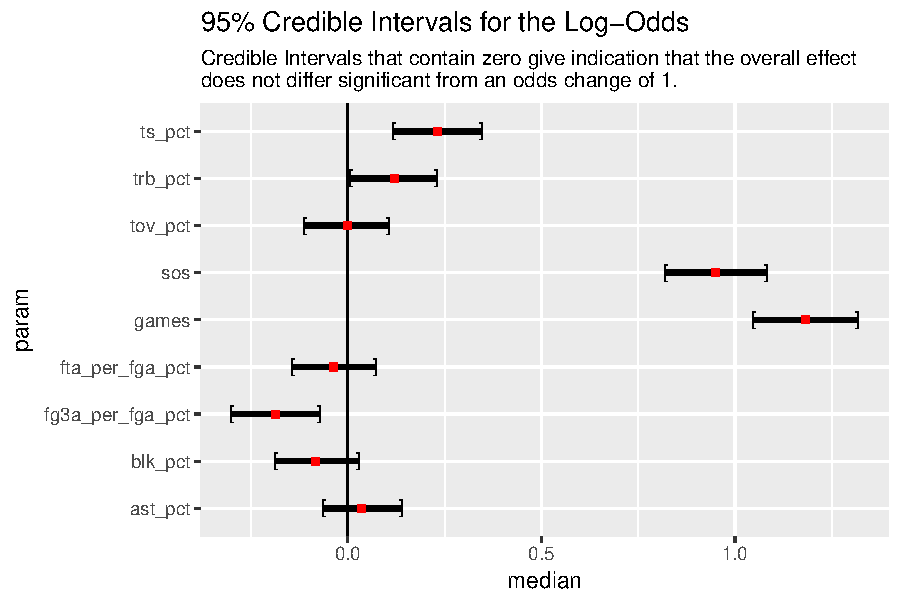
\includegraphics[width=1\linewidth]{../fig/polr_coef}
	\caption{The standard errors, after removing the collinear variables is far more manageable.}
	\label{fig:polr_coef}
\end{figure}

%\missingfigure{After playing with coefficients, remember that for positive coefficients, increasing the value moves us closer to six and for negative coefficients, we move closer to zero with increasing the value}

\subsubsection{Interpretation of the Coefficients}

We began by looking for those coefficients that do not contain zero in their confidence interval.

\begin{description}
	\item[ts\_pct] Teams that tend to shoot better than other teams tend to have a higher probability of advancing in the tournament. We can see that by increasing our ts\_pct by one standard deviation, we believe that our odds will increase  (with 95\% probability)  between 1.13 times and 1.41 times on average. 
	\item[sos] This is the strength-of-schedule variable. We can see that those teams with a larger strength-of-schedule tend to do far better in the tournament. This is intuitive and is in-line with what we would expect. Teams that are in more difficult conferences and make it to the tournament tend to do very well in the field.  If we increase our strength-of-schedule measure by one standard deviation, we expect our odds of moving to the next level (with 95\% probability) to increase by 2.27 times to 2.94 times.
	\item[games] Teams that tend to play more games throughout the season tend to move higher in the tournament. This is the ``big-team'' effect. Those teams that tend to play more games throughout the season tend to be larger schools with a larger focus on the sport of basketball. Increasing our games played by one standard deviation increases our likelihood (with 95\% probability) between 2.86 times and 3.74 times. 
	\item[fg3a\_per\_fga\_pct] Teams that tend to take a disproportionate number of three pointers tend to do worse in the tournament. This may be a result of the fact that three point shots are high risk, high reward, so teams that take a lot of threes may have difficulty sustaining success over many games. Increasing our amount of threes taken as a percentage of field goals by one standard deviation multiplies our likelihood (with 95\% probability) between 0.74 times and 0.93 times. 
	\item[trb\_pct] Teams that tend to rebound more tend to do better in the tournament. A one standard deviation increase in rebounding percentage multiplies our likelihood (with 95\% probability) between 1.01 times and 1.26 times. 
\end{description}
All of the other coefficients contain zero in their confidence intervals, which indicates to that we do not have significant evidence that these predictors have an effect on the odds of a team making it to the next round of the tournament. Overall, the coefficients that were highly non-zero tend to indicate that better teams do well in the tournament, which is not really a surprise, but the sign of the coefficient on three point attempts per field goal attempt surprised us. 


\subsubsection{In-Sample Predictive Performance}
The in-sample performance of the ordinal regression method is given by the following 7x7 confusion matrix (rows correspond to predicted win totals and columns correspond to actual win totals, with both ranging from 0 to 6). We give the in-sample error not to show our prediction accuracy, but as a method of model checking. Our goal in fitting the ordinal regression model was more inferential than predictive, and the in-sample error is a better indication of the fit of the model than it is a sign of the predictive accuracy of the model. 
\begin{figure}[H]
	\centering
	\input{"../fig/polr_predictions.txt"}
\caption{On the left are the true classes and along the top are the predictions from the ordinal regression analysis using the \textit{argmax} of the posterior to discern what the choice of the Bayesian interpretation of the ordinal regression would predict. We can see that the model is decent at classifying the early rounds. Of the teams that were eliminated in the first round, 636 were classified correctly, 135 were incorrectly classified as winning one game, and 3 were projected to win two games. However, the model also appears downwards biased. We can see that of the teams that won the tournament, the model sometimes only said that they would make it one round, and we can see that the model was not able to identify those teams that made it to the finals easily. There were no teams for which we predicted five rounds of advancement. This class may be very hard to identify in general.}
\end{figure}

In summary, our overall in-sample error rates for ordinal regression are below.
\begin{figure}[H]
	\centering 
	\begin{tabular}{cc}
		\toprule
		Measure Name & Measure\\ 
		\midrule
		Total Number of Games & 1570\\ 
		Prediction=Actual Accuracy & 55.73\%\\ 
		+/- 1 Prediction Accuracy & 89.55\%\\ 
		Prediction $>$ Actual Error Rate & 10.38\%\\ 
		Prediction $<$ Actual Error Rate & 33.89\%\\ 
		\bottomrule
	\end{tabular}
	\caption{For a simple algorithm, the fact that we are seeing over 55\% prediction accuracy on a seven-dimensional confusion matrix, and achieving almost 90\% accuracy on a plus / minus one prediction basis on very noisy data set is an accomplishment in and of itself. The downward bias of the model is evident in the fact that almost 34\% of the predictions were under the actual result, and so this is something that we will need to take into account when using the model for prediction}
\end{figure}









%\begin{figure}
%	\centering
%	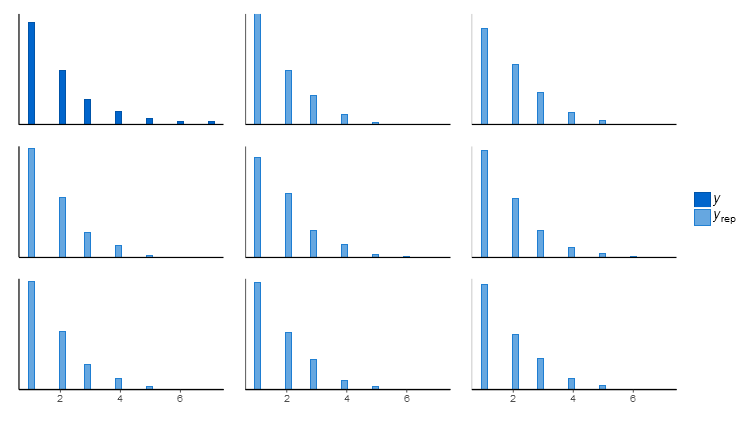
\includegraphics[width=1\linewidth]{../fig/polr_pp}
%	\caption{The upper left histogram is the true distribution of the factor levels of $y$. We can see that their are seven levels - each one half the size of the preceding bar since a team either makes it or does not make it to the next round. We can see that the posterior predictive distributions more or less seem to capture this well, but we can see that for levels greater than four (i.e. for teams that made it to the final four) the ordinal regression model fails to predict well in these tails. As a result, this may be something that we need to correct for when looking at the final four contenders.}
%	\label{fig:polr_pp}
%\end{figure}




%\begin{figure}[H]
%	\centering
%	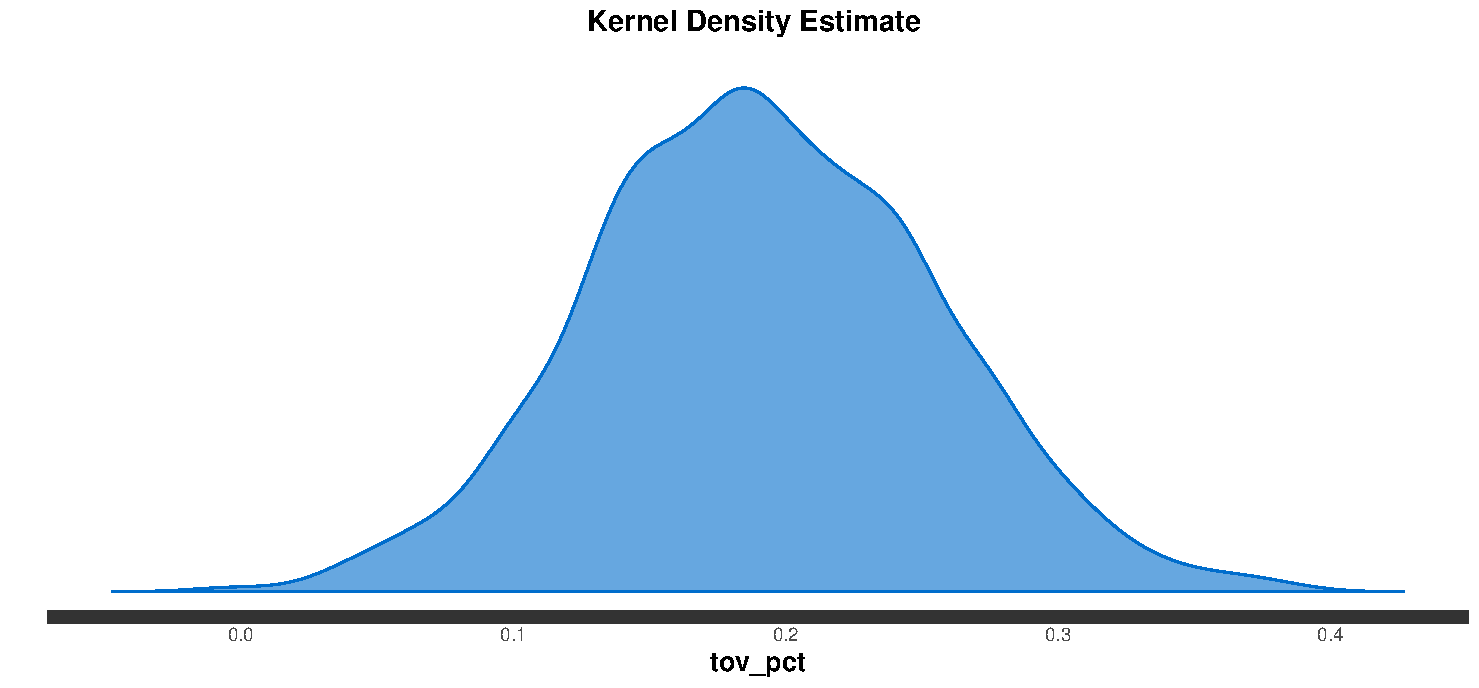
\includegraphics[width=0.7\linewidth]{../fig/polr_tovpct}
%	\caption{The turn-over percentage(tov\_pct) has a positive coefficient which makes sense in the context of the problem. For every standard deviation that a team turns over the ball more than the field on average, we see about a 19\% change in the odds that they lose. This is significant and is in-line with intuition that turnovers can be the critical factor in a tight game in the tournament}
%	\label{fig:polrtovpct}
%\end{figure}

%\begin{figure}[H]
%	\centering
%	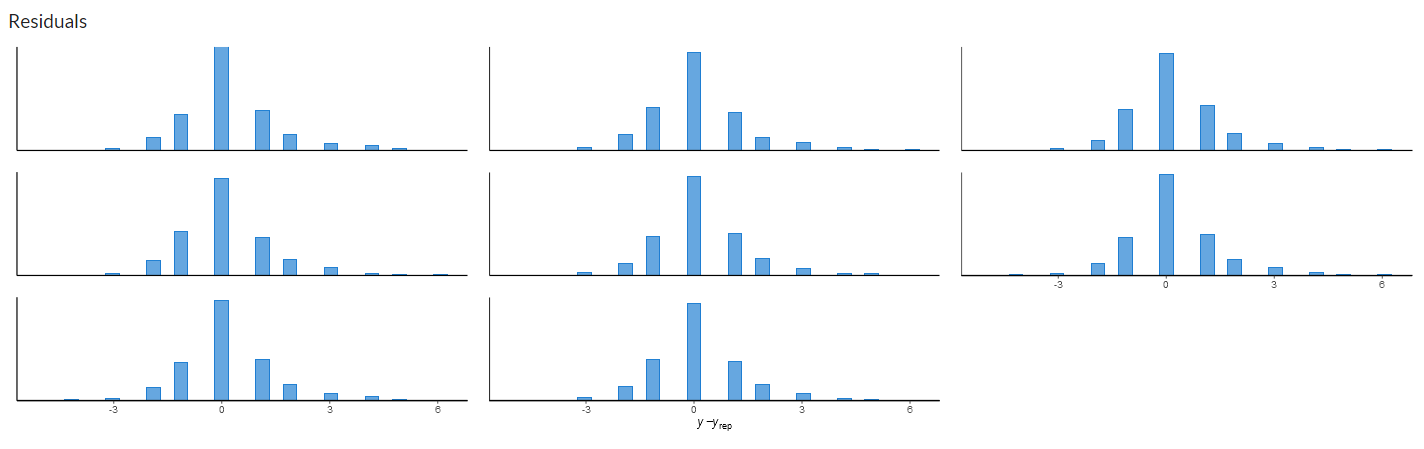
\includegraphics[width=1\linewidth]{../fig/polr_residuals}
%	\caption{captionhere}
%	\label{fig:residuals}
%\end{figure}

%\missingfigure{Still under construction :) - include the results of working with the names model}

% Need to include these!!!!!!!!!!!!!!!!!!
%\begin{figure}[H]
%	\centering
%	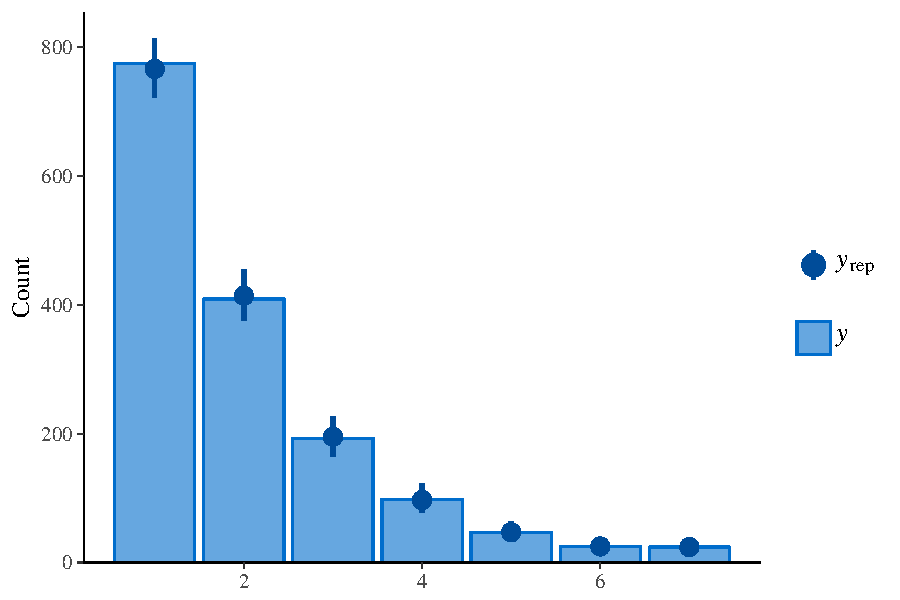
\includegraphics[width=0.7\linewidth]{../fig/polr_name_pp}
%	\caption{If we include the names as variables, we can see that the posterior predictive distribution frequency count is almost spot on with what we observe. This makes sense that our predictions would get better accounting for the individual team variability in the model, but we need to find out if the prediction that comes from this model is something that outperforms the simpler model and is not bias downwards on the predictions of how many people are going to make the tournament, but it is not a drastically improved fit.}
%	\label{fig:polrnamepp}
%\end{figure}
%
%\begin{figure}[H]
%	\centering
%	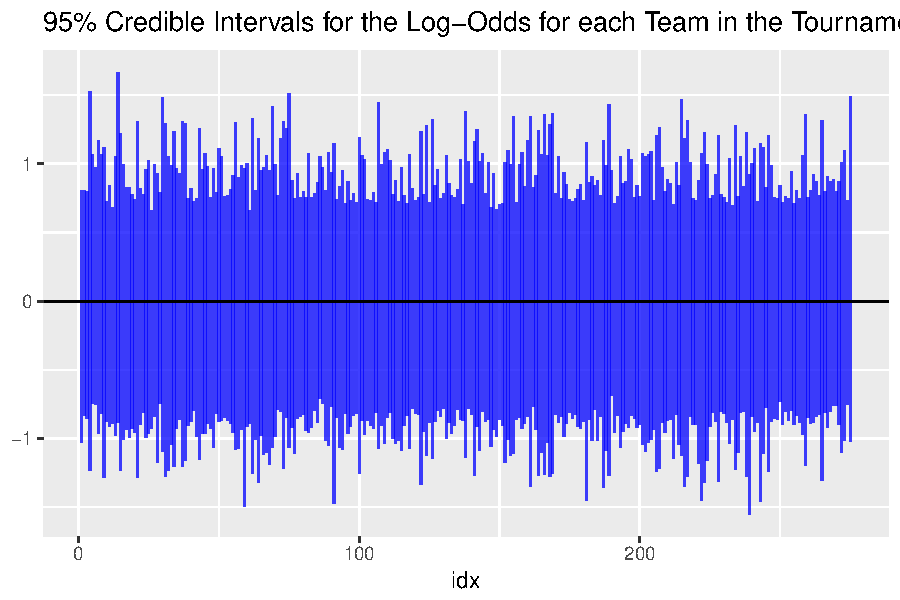
\includegraphics[width=0.7\linewidth]{../fig/polr_team_log_odds}
%	\caption{We can see that the 95\% posterior interval for each of the teams is centered around, and contains zero. This is an indication that for no team in the tournament does their name, controlling for things like shooting percentage performance, account for over or under performance. This finding was highly surprising to us, as we expected certain powerhouse schools like Kentucky to outperform other schools systemically in the tournament but we can see that even the powerhouse teams rely on the fundamentals just as much as everyone else.}
%	\label{fig:polrteamlogodds}
%\end{figure}


\section{Ensemble Prediction Model}
\subsection{Introduction}

We have now seen the predictive ability in both ordinal regression and in some of the methods introduced in the data-exploration. Having looked at the problem for some time, and made inferences about the parameters and the way that the data interacts with how far someone goes in the tournament, we now look for a potential black-box model that may be able to outperform the native methods in terms of predictive accuracy. 

This section aims to detail the search for that model and the methods employed to get the most predictive accuracy that we can out of several models. We aim to use an ensemble model to bring in multiple players into the act, and our hope is that this model can outperform the methods that we have already seen thus far. 

\subsection{Discussion of Stacking}

\textit{Stacking} is a type of ensemble model that aims to combine the outputs of several models that exhibit low to medium correlation and produce estimates that are better than any of the models that it was produced from. The idea of stacking is follows:

\newcommand{\dattrain}{\ensuremath{Data_{train}}\xspace}
\newcommand{\datval}{\ensuremath{Data_{validation}}\xspace}
\newcommand{\dattest}{\ensuremath{Data_{test}}\xspace}
\newcommand{\dattestpreds}{\ensuremath{Data_{test + preds}}\xspace}
\newcommand{\datvaltest}{\ensuremath{Data_{validation + preds}}\xspace}

\begin{enumerate}
	\item Break the data into three pieces: 
	\begin{enumerate}
		\item Training Data (\dattrain) 
		\item Validation Data (\datval)
		\item Testing Data (\dattest)
	\end{enumerate}
	\item Build up $M$ different models on \dattrain. These can be Neural Nets, SVM, Ordinal Regression, Random Forests, etc. Models with different parameters count as ``different'' models.
	\item Out of the $M$ models, find $k$ so called $m^{\star}$ models that exhibit relatively low correlation (in prediction on \dattrain)
	\item Once we have selected our $k$ $m^{\star}$ models, we then concatenate our data to the prediction results of the $m^{\star}$ models on \datval. We will produce a dataframe that looks as follows (named \datvaltest):
	\begin{align*}
	\begin{array}{|c|cccc|}
		\toprule
		\text{Data} & \text{Prediction 1} & \text{Prediction 2} & \cdots & \text{Prediction k} \\ 
		\midrule
		- \datval - & m_1^{\star}(\datval) & m_2^{\star}(\datval) & \cdots & m_k^{\star}(\datval) \\ 
		\vdots & \vdots & \vdots & \vdots & \vdots\\
		\bottomrule
	\end{array} 
	\end{align*}
	\item Train a ``stacker'' model (usually just a regression model but this can be a more complex model as well) on \datvaltest . This model is combining the prediction of the simpler models into a weighed vote which is the output of the stacked model. The goal is to create a classifier that is able to combine the strengths of a bunch of smaller models into a strong classifier. It does so by finding the ``expert model'' for each subset of the data and up-weighting this models prediction in its ensemble vote.
	\item Use the stacked classifier as well as the $m^{\star}$ models to make predictions for \dattest
\end{enumerate} 

\subsection{Visual Depiction of Stacking}
\begin{figure}[H]
	\centering
	\begin{forest}
		[Final Predictions [\dattestpreds [\dattest] [$m^\star_1$ [\dattrain]] [$m^\star_2$ [\dattrain] ][$\cdots$][$m^\star_k$ [\dattrain]]] [Stacked Model [\datvaltest [\datval] [$m^\star_1$ [\dattrain]][$\cdots$][$m^\star_k$ [\dattrain]]] ]]
	\end{forest}
\caption{A visual layout of the way that a stacked model is created. By choosing models with low correlation to build off of, the stacked model is able to find which model is the ``expert'' in a given subregion of the data and up-weight the output of that model in its ensemble prediction. We then use these micro-models, in combination with the stacked model, to make predictions. }
\end{figure}



\subsection{Discussion of Implementation}
For the stacked model, we choose to use the following components as our sub models:
\begin{description}
	\item [Random Forests] varying the number of variables to sample for the trees and the maximum number of nodes
	\item [Decision Trees] varying the number of variables to use for the decisions, the maximum depth of the tree, and the minimum splitting criterion
	\item [Ordinal Regression] varying the link function between logistic, probit, and loglog
	\item [Multinomial Regression] with no variations
	\item [SVM] with linear, radial, and polynomial kernels, varying the cost and gamma parameters
	\item [Adaboost + Bagging] varying the number of iterations, and the algorithm used to determine the coefficients learning algorithm
\end{description}

Then the algorithm proceeds as follows
\begin{figure}[H]
	\centering
	\begin{tcolorbox}
		\begin{algorithmic}
			\State Split Data into \dattrain, \datval, and \dattest
			\ForAll{$m \in Models$}
			\State Train $m$ on \dattrain to get $m^{\star}$
			\State \datvaltest $\leftarrow$ $Predict(m^{\star},\datval)$
			\State \dattestpreds $\leftarrow$ $Predict(m^{\star},\dattest)$
			\EndFor
			%		
			%		\State \Comment{Now \datvaltest and \dattestpreds have the original validation and testing data respectability as well as each models predictions}
			\State BestModels $\leftarrow $ empty
			\State nPredictors $\leftarrow$ 20
			\For{1 $\rightarrow$ nPredictors}
			\If{size(BestModels) == 0}
			\State Find the most accurate model on \datval and \State put it in BestModels
			\Else 
				\State Find a model that predicts well  on \datval \State and is correlated small with models in BestModels.  \State Put it in BestModels.
			\EndIf
			\EndFor
			\State Remove all model predictions in \datvaltest for models $\notin$ BestModels\\
			\State Remove all model predictions in \dattestpreds for models $\notin$ BestModels\\
			\State Train Stacked Model $\hat{SM}$ on \datvaltest\\
			\State Final Predictions $\leftarrow Predict(\hat{SM}, \dattestpreds) $
		\end{algorithmic}
	\end{tcolorbox}
\caption{Implementation of the Stacking Model Algorithm}
\end{figure}




\subsection{Stacked Model Results}

\begin{figure}[H]
	\centering
	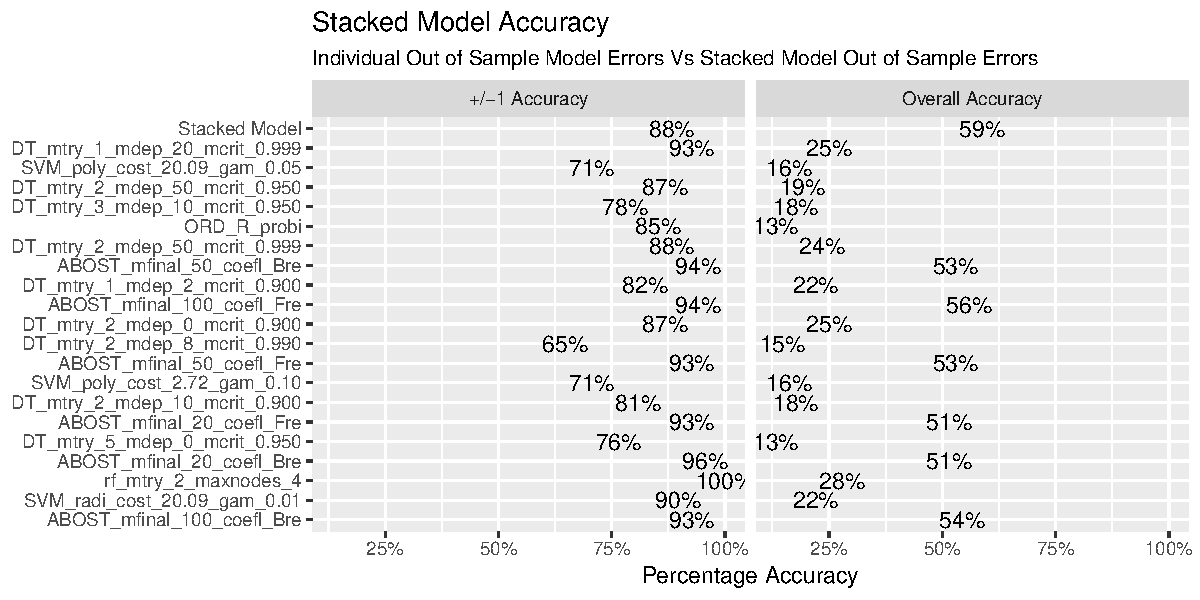
\includegraphics[width=1\linewidth]{../fig/StackedModelAccuracy}
	\caption{We can see a few trends in this graph. On the left axis, we can see the stacked model is the first row, and each row under it is one of the submodels. On the right pane, we have the out-of-sample prediction accuracy on the test data with the stacked model and the sub models. We can see that the sub-model greatly outperforms each of the submodels in terms of accuracy. With an accuracy of 63\%, it manages to correct the bias in each of the sub models and perform far better than any of the models that it trains off of. The plot on the left shows the accuracy if we consider $\pm 1$ as an accurate prediction. We include this metric since this is how many NCAA brackets are graded. For example, a hit would be: in reality a team makes it to the third round and we predict either a second round, third round, or forth round survival rate.}
	\label{fig:stackedmodelaccuracy}
\end{figure}

\begin{figure}[H]
	\centering
	\input{../fig/StackedConfMatrix.txt}
	\caption{The stacked model managed to get the winner of the tournament as well as $\nicefrac{25}{32}$ of the first round losses. The prediction is accurate 63\% of the time (going down the diagonal) and 91\% accurate if you consider the $\pm 1$ prediction band}
\end{figure}


The stacked model does an amazing job at capitalizing on the structure of the submodels and improving their out-of-sample prediction accuracy. This performance is greater than what we expected, but we should not be too surprised after we consider the $\pm1$ accuracy of each of the sub models. 

We can see that each of the sub models was only off by one in either direction. By training a model that can correct their individual bias, we should expect that an ensemble model would be able to outperform any of the candidate models that the stacked model was trained on. 

\section{Conclusion and Further Research}

Having explored a variety of methods, we have founds a number of insights that we feel are important to state here:
\begin{description}
	\item[Stacking is Powerful] Taking a collection of smaller and weakly correlated models and training models that combines them is a powerful idea. The simplicity of stacking (conceptually) and the ease of implementation is something that we will keep in mind. This is a popular technique on Kaggle and it produced amazing results on our test data.
	\item[Three Point Attempts Are Desperate] If we revisit the ordinal regression, we find that those teams that attempt more three pointers as a percentage of their field goals typically did worse in the tournament. This came as a surprise but makes sense given the nature of those teams that typically attempt a lot of three pointers - they are typically down in the tournament.  
	\item[Other] \missingfigure{Eli and Andrei!!!}
\end{description}




\newpage
\begin{thebibliography}{9}
	
	\bibitem{bballsite}
	“NCAA Tournament History.” Edited by Sports Reference LLC, College Basketball at Sports-Reference.com, {\color{blue} \url{www.sports-reference.com/cbb/postseason/}}.
	
\end{thebibliography}



\end{document}
